
%-----------------------------------

\documentclass[english]{article}
\usepackage[T1]{fontenc}
\usepackage{pslatex}
\usepackage[latin9]{inputenc}
\usepackage[a4paper]{geometry}
\geometry{tmargin=2.5cm,bmargin=2.5cm,lmargin=2.5cm,rmargin=2.5cm}
\usepackage{textcomp}
\usepackage{amssymb, amsmath,stmaryrd}
\usepackage[english]{babel}
\usepackage{listings}
\usepackage{graphicx,float}
\usepackage{lastpage}
\usepackage{hyperref}
\usepackage[anythingbreaks]{breakurl}
\usepackage{fancyhdr}
\usepackage{listings}
\usepackage{color} 

%-----------------------------------

\makeatletter % to deal with @ in Latex code. see http://tex.stackexchange.com/questions/8351/what-do-makeatletter-and-makeatother-do

\pagestyle{fancy}
\fancyhf{} 

\newcommand{\matiere}[1]{\def\@matiere{#1}}

\newcommand{\depart}[1]{\def\@depart{#1}}

\newcommand{\module}[1]{\def\@module{#1}}

\makeatletter
\def\maketitle{
	\hypersetup{%
		pdftitle={\@title}, 
		pdfauthor={\@author},
		pdfsubject={\@matiere},
		pdfborder = {0 0 0}
	}%
	
	\thispagestyle{plain}
	\begin{center}
		{\Large \@matiere}
		\vskip 0.3cm
		\rule[0.5ex]{\textwidth}{0.4pt}
		\vskip 0.4cm
		{\LARGE \bf \@title}
		\vskip 1cm
	\end{center}
}


\fancyhead[L]{\footnotesize{\@title}}
%\fancyhead[L]{\footnotesize{\@module}}
\fancyhead[R]{\footnotesize{\@matiere}}
\fancyfoot[L]{\footnotesize{\textit{\@depart}}}
\fancyfoot[R]{\footnotesize{\thepage/\pageref{LastPage}}}
\renewcommand{\headrulewidth}{0.4pt}
\renewcommand{\footrulewidth}{0.4pt}

\fancypagestyle{plain}{%
	\fancyhf{} 
	\fancyfoot[R]{\footnotesize{\thepage/\pageref{LastPage}}} 
	\fancyfoot[L]{\footnotesize{\textit{\@depart}}}
	\renewcommand{\headrulewidth}{0pt}
	\renewcommand{\footrulewidth}{0.4pt}}

\newenvironment{q}{
	\begin{enumerate}
		\setlength{\itemsep}{1pt}
		\setlength{\parskip}{0pt}
		\setlength{\parsep}{0pt}}
	{\end{enumerate}
}


%------------------------------

\definecolor{mygreen}{rgb}{0,0.6,0}
\definecolor{mygray}{rgb}{0.5,0.5,0.5}
\definecolor{mypurple}{rgb}{0.58,0,0.82}

\lstset{ %
	backgroundcolor=\color{white},   % choose the background color; you must add \usepackage{color} or \usepackage{xcolor}
	basicstyle= \small\ttfamily,     % the size of the fonts that are used for the code \tiny for smaller font
	breakatwhitespace=false,         % sets if automatic breaks should only happen at whitespace
	breaklines=true,                 % sets automatic line breaking
	captionpos=b,                    % sets the caption-position to bottom
	commentstyle=\color{mygreen},    % comment style
	deletekeywords={...},            % if you want to delete keywords from the given language
	escapeinside={\%*}{*)},          % if you want to add LaTeX within your code
	extendedchars=true,              % lets you use non-ASCII characters; for 8-bits encodings only, does not work with UTF-8
	frame=single,                    % adds a frame around the code
	keepspaces=true,                 % keeps spaces in text, useful for keeping indentation of code (possibly needs columns=flexible)
	keywordstyle=\color{blue},       % keyword style
	language=C++,                 % the language of the code
	morekeywords={*,...},            % if you want to add more keywords to the set
	numbers=none,                    % where to put the line-numbers; possible values are (none, left, right)
	numbersep=5pt,                   % how far the line-numbers are from the code
	numberstyle=\tiny\color{mygray}, % the style that is used for the line-numbers
	rulecolor=\color{black},         % if not set, the frame-color may be changed on line-breaks within not-black text (e.g. comments (green here))
	showspaces=false,                % show spaces everywhere adding particular underscores; it overrides 'showstringspaces'
	showstringspaces=false,          % underline spaces within strings only
	showtabs=false,                  % show tabs within strings adding particular underscores
	stepnumber=1,                    % the step between two line-numbers. If it's 1, each line will be numbered
	stringstyle=\color{mypurple},     % string literal style
	tabsize=2,                       % sets default tabsize to 2 spaces
	title=\lstname                   % show the filename of files included with \lstinputlisting; also try caption instead of title
}



\makeatother 
%--------------------------------------------------------------------------------


\begin{document}
	
\begin{center}
	\Huge\textbf{Khoi Pham Nhat}
\end{center}
	
{\matiere{Bachelor in Robotic and Computer Vision}
		
\title{C++ Project report}
	
\depart{Centre Universitaire Condorcet - Bachelor in Computer Vision 2016/2017}
		
\maketitle 

\includegraphics[width=15cm,height=13cm]{img/about.JPG}

\newpage 
	
\tableofcontents
		
\newpage 
		
		
		
		
\section{Knowledge and techniques used in the project}

Here I list all the C++ techniques that have been used throughout the project in order to have a general overview on C++ functions, strengths and rules; so I could be able to build the plan to achieve the goal.

\subsection{Data type, variable and scope}
	
	\begin{itemize}
		\item Data type conversion/casting
		
		Data type in C++ is numerous and need to be used in right place and time to reduce oversize container issue which means "takes up space that doesn't require to". In general, data types of programing language, born to category, give focal point on a specific case so that it speeds up the process, data type in C++ share the same idea.
		
		Quick look on Data type casting: to switch a variable from one data type to another, to be able to use power of that certain data type.
		
		\lstset{language=C++}
		\begin{lstlisting}
		
			// cast variable m from int to double to have ability to  
			// store the fractional result of its division with 3
			int m = 2;
			double n = (double)m/3;
		\end{lstlisting}
		
		\item Variable and scope
		
		Variable is an object/instance of a certain data type/class that stores something has that type of data or class. We use variable to carry the information throughout a program.
		
		And scope, is a concept in programing to limit this transportation scope/range of a variable.
		
		\lstset{language=C++}
		\begin{lstlisting}
			
			// x is in parent scope compare to function1 and function2
			// then these 2 functions can used x in their scope. On the other
			// hands, b belongs only in function 1 scope, function2 couldn't
			// be using it like in this example and will cause an error.
			int x = 5;
			
			int function1 () {
				int a = 10;
				int b = 5;
				return x+a+b; // return 20;
			}
			
			int function2 () {
				int a = 10;
				return x+a+b; // return error undefined b;
			}
		\end{lstlisting}
		
	\end{itemize}
\newpage


\subsection{Built-in and customized functions}
	\begin{itemize}
		\item Function
		
		The usage of function in general, is to pack a block of code that made to solve a certain task in a program. Any function in C++ all belongs to a certain class, and will be called within the domain of this class.
		
		Function is also a key to access and manipulate a private property of a class.
		
		\item Return
		
		"return" is a powerful keyword in C++ which is a tool to transport the output of a function to the outside world so that user can manipulate or store it after the end of a function life.
		 
		\lstset{language=C++}
		\begin{lstlisting}
		
			int x = 5;
			
			int function1 () {
				int a = 10;
				int b = 5;
				return x+a+b; // return 20;
			}
			
			int y = function1(); // y now has value of 20
		\end{lstlisting}
	\end{itemize}



\subsection{Condition statement}

	If statement somehow share the same idea with data types and scope in term of purpose which is supposed to category and narrow down the case of a value or a set of value, redirect the process flow based on the natural or characteristic of these values. 
	
	\lstset{language=C++}
	\begin{lstlisting}
		
		int function1 () {
			int a = 10;
			int b = 5;
			return a+b; // return 20;
		}
		
		// stop or keep processing depending on value of function1
		if(function1 < 10) return;  
	\end{lstlisting}


\subsection{List, array, vector and struct}
	
	These are main containers in C++ to describe a set of a certain data types / classes. These containers not only store the data but also provide a variety method to manipulate these data. This is perfect idea to group and solve mass problems at once, without losing track and consistency. 
	
	
	\begin{itemize}
		\item Array
		
		Array is more lighter than the rests, we can access elements inside an array easily, inexpensively. However, array is fixed size container, that means once it already born, we can not add more element later. 
		
		\lstset{language=C++}
		\begin{lstlisting}
		
			// create an array of integer
			int array[] = {16,2,77,29};
		\end{lstlisting}
	\end{itemize}
	
	
	\begin{itemize}
		\item List
		
		List on the other hand of Array, is dynamically created and element assigned, but lose the advantage of picking a random element inside it. This could be done but with much more cost.
		
		\lstset{language=C++}
		\begin{lstlisting}
		
			// create a list of integer
			std::list<int> l = {16,2,77,29};
		\end{lstlisting}
		
	\end{itemize}


	\begin{itemize}
		\item Vector
		
		Vector is expensive, take much space, in order to merge 2 advantage of list and array, to come up with a responsive container but also requires less effort extracting the element.
		
		\lstset{language=C++}
		\begin{lstlisting}
		
			// create a vector of integer
			std::vector<int> v = {16,2,77,29};
		\end{lstlisting}
	\end{itemize}
	
	\begin{itemize}
		\item Struct
		
		A data structure is a group of data types grouped together under one name. There is a more advance form of this called Class, however, this container is more suitable dealing with simple problems.
		
		\lstset{language=C++}
		\begin{lstlisting}
		
			struct Cat {
				int age;
				QString name;
			};
			
			Cat blackCat, ArabCat
		\end{lstlisting}
	\end{itemize}



\subsection{Loops}

	\begin{itemize}
		\item For loop:
		
		Mass data processing tool, programing language is strong in automate data manipulating in order to perform and realize both simple and complicated algorithms supposed to solve a certain problem. 
		
		For loop is nothing more than a scanner with a controllable in data range picking and frequency (customized index increment).
		
		\item While loop:
		
		Share same main idea with For loop, the difference is While loop has only condition to loop, while needs no range, nor index. Therefore, will be used to solve simple looping processes.
		
		
	\end{itemize}

\newpage

\subsection{Pointer}

Pointer was born to reduce the effort of the machine trying to locate data in memory hence speed up processing time of the program. Without pointer, basically it's should be no matter, the program works fine without pointer until a heavy workload task get involved.

The idea of pointer is to store the address of a block memory rather than its value. Therefore, the connection and transport process between 2 location in a thread of the processor is less heavy since the weight of an address (in most case) lighter than an object.

\begin{center}
	\includegraphics[width=8cm,height=6cm]{img/pointer.png}	
\end{center}	

\lstset{language=C++}
\begin{lstlisting}

	int val = 5;
	int *ptr = &val;
	
	cout << ptr ; // will print 0xFE
	cout << *ptr ; // will print 5
	
\end{lstlisting}


\subsection{Class}
	
	C++ world was built based on Classes and its relationship (inheritance), It is the most well known technique in OOP programing which used to category, characterize, build and manipulate different kind of data in an abstract way. It's also known as the prototype of the program, a sketch to build up structure of the whole architect design. 
	
	\begin{itemize}
		\item Attribute
		
		Properties of a class, these are merely variables to store a specific data that build the class characteristic.
		
		\item Constructor and Destructor
		
		Constructor and destructor are 2 special Class functions, one creates an instance of the class and one kills it.
		
		The Attribute could be created at the same time when the instance was born by passing values onto Constructor
		  
		\item Accessor and mutator
		
		Accessor is the key to outside world to see what inside a class which was set to private or protected status. While mutator has power to flash it with new values. 
		
		\item Function and Class function
		
		Function in a class will only be used by members of the class, to get, change and manipulate data inside that member. Accessor and mutator are also function but only to serve simple purposes (get and change an attribute). Normal function in general is more designed to manipulate data instead.
		
		Class function is the same with normal function, but they are called upon the Class itself, not from an instance/object of that class. 
		
		\lstset{language=C++}
		\begin{lstlisting}
		
			// this function is called from QPixmap Class, very handy in
			// such cases of conversion / transform between classes
			QPixmap::fromImage(QImage);
		\end{lstlisting}
		
	\end{itemize}



\subsection{QT UI and utils}

	QT is a powerful framework that provides tons of cool Classes with hundreds of built-in functions for programmer to build a program with less effort, time consuming and not to reinvent the wheel.

	\begin{itemize}
		\item QColor, QRgb
		
		These two classes deals with pixel color, help us read values from every color channels of a pixel. Therefore, we don't need to loop through the 4 dimension matrix of every pixel to be able to get its value.
		
		\item QImage, QPixmap
		
		QImage and QPixmap somehow share similar functions and both used to store image data. These are 2 main Classes we used to manipulate image in QT.
		
		\item QPainter
		
		QPainter is really a painter! (surprised). It is actually a virtual pencil/brush like tools in photoshop to draw graphical output, it has preset option like stroke, color, coordinators, etc, for us to display what we want to be displayed in the canvas.
		
		\item QLabel, QPushButton, QCheckBox, etc
		
		These are QT UI components class for us to make ui components like we usually see in software or website like label, button, sliders, etc.
		
	\end{itemize}



\newpage


\section{Method and approaches}

To achieve this project of Pixel Art, I've created considerably many functions and ideas that made the program way more complex but also more efficient, handy and well performance. \newline

Therefore, I break it down into categories with a good logic way to catch the general ideas as well as distinguishing the main and extras features. \newline

Please note all the codes written below may not be exactly the same in c++ files since I removed redundant parts and leave the main necessary parts only that express my ideas the best. Here is the list of all functions in the program:
\subsection{Main functions}

\subsubsection{Load button}
Very simple function where I load an image using QFileDialog with an absolute default location url and image extension filters.


\lstset{language=C++}
\begin{lstlisting}	
	filePath = QFileDialog::getOpenFileName(
							this,		// set parent of this class is mainWindow
							"Select an image",
							"d:\\CProject/PixelArt",
							"Images (*.png *.jpg *.jpeg)");
							
		
\end{lstlisting}

A simple return condition in case the user didn't choose the file (if the program keeps proceeding it will get error since the value of the file variable is empty) 


\lstset{language=C++}
\begin{lstlisting}
	if (filePath.isEmpty()) return;
	
	
\end{lstlisting}

A pixmap created using the received url and passed onto a QGraphicView viewport to show it on the screen. By creating an instance of QGraphicsScene, we add the pixmap and set it to link with the corresponding UI component name pictureViewport.

\lstset{language=C++}
\begin{lstlisting}
	img = new QImage(filePath);
	pixmap = new QPixmap;
	*pixmap = QPixmap ::fromImage(img);
	
	// QGraphicView config, this block of code is inside updateViewport(QImage)
	// function, this function will be used instead for the rest of the document
	pictureViewport     = new QGraphicsScene;
	pictureViewport     ->addPixmap(*pixmap);
	
	ui->pictureViewport ->setScene(pictureViewport);
	ui->pictureViewport ->show();
	
	
\end{lstlisting}


\subsubsection{Pixelize button}

Overview: 

\begin{itemize}
	\item The Pixelize button read through the image matrix, create a virtual window by a given size (using step increment of loops), I called it pixel \textbf{CUBE}. 
	
	\item Another pair of loops scan through every pixel inside each cube to grab color value and do Mean value computation 
	
	\item Assign calculated Mean value back to every pixel within the cube.
	
	\item Update the viewport with the processed image. 
	
\end{itemize}

\newpage

\lstset{language=C++}

\begin{lstlisting}

	// create a virtual window by the given sizes
	// note that these loop parameters had been normalized:
	// rows = imgWidth/size cols = imgHeight/size
	// for loop before normalizing: for(int i=0; i<imgWidth; i+size)
	for(int i = 0; i < rows; ++i)
	for(int j = 0; j < cols; ++j){
	
		// loop through every pixels of the pixel cube
		for(int k = 0; k < cubeH; ++k)
		for(int l = 0; l < cubeW; ++l){
			.. extracting color value from pixel
		}
		
		Mean calculating.. 
		
		// loop through every pixels of the pixel cube again
		for(int k = 0; k < cubeH; ++k)
		for(int l = 0; l < cubeW; ++l){
			.. assign back color value on to pixel
		}	
	}
	
	// update viewport
	updateViewport(pixelizedImg);
\end{lstlisting}




\subsubsection{Art it button}

Overview: 

\begin{enumerate}
	\item Open Directory from user computer to load multiple sample image files, store them in a vector.
	
	\item Calculate mean color value of each of these sample images, store them in another vector.
	
	\item Loop through all the virtual cubes as mentioned in pixelizing function, for each cube, compare its mean color value with mean color values of sample images to find the best matched one (This is where the hell begin!). 
	
	\item Draw the best matched image onto the position of the cube.
	
	\item Update the viewport with the processed image. 
	\newline
\end{enumerate} 



\textbf{1/ Load multiple images} \newline

\lstset{language=C++}
\begin{lstlisting}

	// Get sample image folder absolute path using QFileDialog::getExistingDirectory
	QString dirPath = QFileDialog::getExistingDirectory(
								this,
								"Select sample images",
								"d:\\CProject/PixelArt",
								QFileDialog::ShowDirsOnly); // see folder only mode
						
	// create QDir using the path							
	QDir dir(dirPath); 
	
	// filter the QDir to load only .jpg and .png files
	dir.setNameFilters(QStringList()<<"*.jpg" <<"*.png"); 
	
	// extract relative path of all images inside QDir
	QStringList relativePaths = dir.entryList();
	
	// create the images using the file paths and add them to a vector
	for (int i =0; i < relativePaths.size(); i++){
	
		// convert relative path to absolute path to use it to create QImage
		QString absImgPath = dir.absoluteFilePath(relativePaths[i]);
		QImage *image = new QImage(absImgPath);
		
		imgList.append(image);	// add the image to the vector
	}
	
\end{lstlisting}


\textbf{2/ Sample images mean color processing} \newline
\lstset{language=C++}
\begin{lstlisting}

	QVector<QImage*>::iterator sampleImage;
	
	// loop through image list using qvector iterator
	for(sampleImage = imgList.begin(); sampleImage != imgList.end(); ++sampleImage){
	
		int count = 0, red = 0, green = 0, blue = 0, alpha = 0;

		// find the most representative color from images
		// as what happened in pixelizing image function
		for(int m = mark1; m < mark2; ++m)
			for(int n = mark3; n < mark4; ++n){
			
				// convert the QRgb to QColor for color extracting process
				QColor color((*sampleImage)->pixel(m,n));
				
				red += color.red();
				green += color.green();
				blue += color.blue();
				alpha += color.alpha();
				
				// count the iteration to get the total pixel of the cube
				count++;
			}
		
		// calculate mean color value of every channels
		red /= count; green /= count; blue /= count; alpha /= count;
		
		// store this combination of color in the sample color list
		sampleColorList.append(QColor::fromRgba(qRgba(red,green, blue,alpha)));
	}

\end{lstlisting}


\textbf{3/ Find best matched image of each window} \newline

This task is consisted of 3 children task to be accomplished, including: \newline\newline
	\textbf{A/} Create a class to represent the previously mentioned cubes, transform them from virtual objects to real objects. Therefore we could be able to play with them later, and most importantly to store them and its necessary properties.

\lstset{language=C++}
\begin{lstlisting}
	
	class PixelCube
	{
	public:
		PixelCube();
		PixelCube(int red, int green, int blue, int alpha){
			r = red; g = green; b = blue; a = alpha;
		}
		
		// function to find the best matched index in a list of
		// sample colors (extracted from the multiple sample images)
		int findBestMatchedIndex(QVector<QColor> sampleColors);
		
	private:
		int r, g, b, a;
		int w, h;
	};

\end{lstlisting}

This class stores the 4 color values of the cube, and 2 dimensions. \newline\newline
\textbf{Remark}: the purpose of storing 2 dimensions is that not all the times all the cubes have the same dimensions. This happens with cubes at the right and bottom edges of the image where they got cut partially in size.\newline\newline
Next step, I created the instance of this class and pass in those needed values by the moment I virtually created them in Pixelizing process.

\lstset{language=C++}
\begin{lstlisting}
	pixelizing function(){
		...
		
		// calculate mean color value of every channels
		r /= count; g /= count; b /= count; a /= count;
	
		// transform this block of pixel as an instance of PixelCube for PixelArt function
		PixelCube *newcube = new PixelCube(r,g,b,a);
		
		// set width height for this cube
		newcube->setWidth(cubeWidth);
		newcube->setHeight(cubeHeight);
		
		// store this PixelCube in Grid using the "normalized" i and j indexes
		setPixelCube(i, j, *newcube);
		
	}
\end{lstlisting}

Grid in the piece of code above is a 2 dimensions vector I created as mainWindow's property in order to store these PixelCube instances.

\lstset{language=C++}
\begin{lstlisting}
	std :: vector < std :: vector < PixelCube > > grid; // store blocks of pixel
	
	/* accessors */
	PixelCube& getPixelCube (int i, int j) {
		assert( i < rows && j < cols ); return grid[i][j];
	}
	
	/* mutators */
	void setPixelCube (const int i, const int j, const PixelCube &cube)  {
		assert( i < rows && j < cols ); grid[i][j] = cube;
	}
\end{lstlisting}  

The Grid represents the shape, size and arrangement of the cubes, most importantly is to store their positions (this ideas I used refer from minesweeper game) so I can use it to position my painter later on. The graph below describes this model.

\begin{center}
	\includegraphics[width=\linewidth,height=7cm]{img/model.jpg}	
\end{center} 


\textbf{B/} Create function for each PixelCube to find best matched image from the vector of sample images. \newline

\lstset{language=C++}
\begin{lstlisting}

int PixelCube::findBestMatchedIndex(QVector<QColor> sampleColors){
	
	// the index of the color that most close to the color of the cube
	int currentBestMatchedIndex;
	
	..
	
	Comparison process..
	
	..
	
	return currentBestMatchedIndex;

}

\end{lstlisting}

I changed the first idea a bit to increase performance of the program: \newline 
From:\newline "Find best matched image from vector of sample images" \newline\newline
To:\newline "Find index (position) of the best matched color (which proportionally the same index with best matched image) from vector of sample image color"\newline

This alternation increase whole lot performance when it reduces the transportation weight of both input and output passing through the function.  \newline

If we pass in a list of image in this function, we have to calculate the mean color of the sample images for every pixel cube which is a stupid duplicate work. This task should be done only once and outside the function. \newline 

That's the reason why by the moment I successfully loaded sample images, I compute all their mean color of and put them in a vector. Now I can use it to pass in this function as a super light parameter storing integer elements. And, since the vector of color has the same size and proportionally relate to the list of images, I definitely can find the best matched image once I have the best match color. \newline

And, below is the the comparison algorithm to find the best match index from the vector of colors

\lstset{language=C++}
\begin{lstlisting}

	// this is a temp variable to store the current shortest distance
	// between the color of the cube and color of sample images. This takes 
	// 255*4 as ini value since 255*4 is the maximum color value of 4 channels
	int currentDiff = 255*4;
	
	// A temp variable to store the index of the color that is most close to 
	// the color of the cube
	int currentBestMatchedIndex;
	
	// declare iteratior (for the loop)
	QVector<QColor>::iterator it;
	
	// loop through sample color list using qvector iterator
	for(it = sampleColors.begin(); it != sampleColors.end(); ++it){
	
		int meanR = 0, meanG = 0, meanB = 0, meanA = 0, totalDiff = 0;
		
		// calculate the difference on all 4 channels
		// by comparing them with these 4 values of the cube
		meanR = abs(r - it->red());
		meanG = abs(g - it->green());
		meanB = abs(b - it->blue());
		meanA = abs(a - it->alpha());
		
		// sum the differences
		totalDiff = meanR + meanG + meanB + meanA;
		
		// set the current difference and the index of the iterator to this case
		// if the difference amount is smaller than the current difference (the
		// smaller the distance is, the more the colors match each others)
		if(totalDiff < currentDiff){
			currentDiff = totalDiff;
			currentBestMatchedIndex = it - sampleColors.begin(); // extract current index
		}
		
	}


\end{lstlisting}


\textbf{C/} Prepare a QPainter \newline

Here is the plan, for every cube in the grid, I find the best match image and definitely I need to show it on the screen. So I choose QPainter to draw and joint those images all together on a new canvas that has the same size with the original image. It'd be like this: 

\lstset{language=C++}
\begin{lstlisting}

	// create a painter to join (by painting) best matched image into a big 
	// canvas in order to have a big combination image after processing
	QPainter cubePainter;
	
	// duplicate new image from pixelized image then use it as a canvas
	artedImg = *pixelizedImg;
	
	// choose the canvas to paint in
	cubePainter.begin(&artedImg);

	// loop through the grid (matrix of cubes)
	for (cubeRow = grid.begin(); cubeRow != grid.end(); ++cubeRow){
	for (cube = cubeRow->begin(); cube != cubeRow->end(); ++cube){
			
			1/ Find best matched image of that cube
			
			2/ Paint that image using the painter:
			
			cubePainter.drawImage(.., bestMatchedImg, ..);

	}
	}
	
	// end painting (close the canvas)
	cubePainter.end();

\end{lstlisting}



\textbf{4/ Draw the processed image } \newline

Apply them all together. We receive the product image by the end of the process and show it on the viewport using updateViewport() function

\lstset{language=C++}
\begin{lstlisting}
	QPainter cubePainter;
	
	artedImg = *pixelizedImg;
	
	cubePainter.begin(&artedImg);
	
	int m = 0;
	for (cubeRow = grid.begin(); cubeRow != grid.end(); ++cubeRow){
		int n=0;
		for (cube = cubeRow->begin(); cube != cubeRow->end(); ++cube){
		
		// passin the sample image color list to find the bestMatchIndex
		// (it's also the index of best match image in the sample
		// image list) of this cube so that we can get the best
		// matched image in sample image list using this index
		QImage *tempImg = imgList[(*cube).findBestMatchedIndex(sampleColorList)];
		
		cubePainter.drawImage(QRectF(n*cubeW,m*cubeH,cubeW,cubeH),
							*tempImg,
							// with this coordinator for source image, painter could be able
							// to take the center region of the image that will be processed
							QRectF(tempImg->width()/2-cubeW/2, tempImg->height()/2-cubeH/2, cubeW, cubeH));
		
		n++; // increase col iterator index	
		}
		m++; // increase row iterator index
	}
	
	// end painting (close the canvas)
	cubePainter.end();

	// update viewport 
	updateViewport(artedImg);

\end{lstlisting}

\newpage

\subsection{Utils/auxiliary functions}

This section consists of helpful functions that I used throughout the program and all extra cool features that I emerge in this project besides 3 main functions above. 

\subsubsection{Centering the program}

A snip-let of code that re-calculate the root for the mainWindow so it could be appeared in the middle of the screen.

\lstset{language=C++}
\begin{lstlisting}

	// get geometry parameters of the screen
	QRect desktopScreen = QApplication::desktop()->screenGeometry();
	
	// new coordinators for mainWindow
	int posX = (desktopScreen.width()-w.width()) / 2;
	int posY = (desktopScreen.height()-w.height()) / 2;
	
	// move the mainWindow by this coordinators
	w.move(posX, posY);
\end{lstlisting}


\subsubsection{Cube size selectors}

Simple ui component to change the value of 2 sizes of the cube in real time.

\begin{center}
	\includegraphics[width=4cm,height=1cm]{img/cubesize.jpg}	
\end{center} 

\lstset{language=C++}
\begin{lstlisting}
	// pixel cube size input
	void MainWindow::on_inputSizeW_editingFinished(){
		cubeW = ui->inputSizeW->value();
	}
	
	void MainWindow::on_inputSizeH_editingFinished(){
		cubeH = ui->inputSizeH->value();
	}
\end{lstlisting}

\begin{center}
	\includegraphics[width=4cm,height=1cm]{img/validator.jpg}	
\end{center} 

Together with it is the user value input validator that will highlight (in red) the QSpinBox that has 0 in value and escape the function until a valid number is inputed.

\lstset{language=C++}
\begin{lstlisting}
	// abort the function if cubesize got 0 in values and highlight the cube size selectors
		if(cubeW == 0 || cubeH == 0){   // we don't care about negative cases since 	QSpinBox takes only positive numbers
		
		if(cubeW == 0){
			ui->inputSizeW->setStyleSheet("QSpinBox { color : red; }");
			ui->inputSizeH->setStyleSheet("QSpinBox { color : black; }");
		}
		
		if(cubeH == 0){
			ui->inputSizeH->setStyleSheet("QSpinBox { color : red; }");
			ui->inputSizeW->setStyleSheet("QSpinBox { color : black; }");
		}
		
		return;
	}else{
		// unhighlight the selectors if the sizes were valid
		ui->inputSizeW->setStyleSheet("QSpinBox { color : black; }");
		ui->inputSizeH->setStyleSheet("QSpinBox { color : black; }");
	}
\end{lstlisting}


\subsubsection{UpdateRowNColAmount}

Throughout the program, there are 2 vectors dynamically created with size according to the dimension of the picture and sizes of the cube. Therefore, they need to be resize every time a new parameter got changed. 

\lstset{language=C++}

\begin{lstlisting}

// empty and resize the vectors
void MainWindow::updateRowNColAmount(QImage &processingImg){
	
	// set number of pixel cubes will be constructed using this
	// image, on both axises. If condition on remainder checking of picture
	// width + cube division will count the rows and cols include the exception
	// case where the cubes are cut by the edge of the window.
	setNumRows(ceil(processingImg.height()  / (double)cubeH));
	setNumCols(ceil(processingImg.width() / (double)cubeW));
	
	// resize (init the size) the grid vector base on the number of cols and rows above
	if(!grid.empty()) grid.clear();
	grid.resize (rows, vector <PixelCube> (cols));
}

\end{lstlisting}


\subsubsection{Introduction/about label}

Impressive Intro label in the middle of the viewport, will be hidden when the first image get loaded.


\begin{center}
	\includegraphics[width=6cm,height=6cm]{img/about.jpg}	
\end{center}  

\lstset{language=C++}
\begin{lstlisting}

	QImage *aboutPage = new QImage();
	
	aboutPage->load("D://CProject/PixelArt/extras/about.jpg");
	
	aboutPage->scaled(496,470);
	
	ui->aboutLabel->setPixmap(QPixmap::fromImage(*aboutPage));

\end{lstlisting}



\subsubsection{Reset button}

This button reloads the original image no matter which image is showing on the viewport. In this function I supposed to used the "img" variable since it's the orignal image, however updateViewport() function doesn't take that image so I re-create the original img using the first filePath. (I have no more time to debug this case, so..)

\lstset{language=C++}
\begin{lstlisting}

	void MainWindow::on_btnReset_clicked(){
	
		img = new QImage(filePath);
		
		// create new pixmap using original image
		updateViewport(*img);
	}
\end{lstlisting}



\subsubsection{Save image}

This button save the image using the absolute path that QFileDialog generate when the user choose saving destination folder.

\lstset{language=C++}
\begin{lstlisting}

	void MainWindow::on_btnSave_clicked(){
		
		QString saveName = QFileDialog::getSaveFileName(this, tr("Save the picture"),
												"",
												tr("Images (*.png *.jpeg *.jpg)"));
		
		curImg->save(saveName);
	}
\end{lstlisting}



\subsubsection{Tracking user behaviors}

1 variable "status" to track down which stage user is on to guide the user to follow the procedure order by enabling/disabling the buttons at a particular stage. This status will be set by the end of a particular function like Load/Pixelize/PixelArt.

\lstset{language=C++}

\begin{lstlisting}

	void MainWindow::on_btnLoad_clicked(){
		...
		status = "loaded";
	}
	
	void MainWindow::on_btnPixelize_clicked(){
		...
		status = "pixelized";
	}

\end{lstlisting}

Enable/disable the buttons according to the status:

\begin{lstlisting}

	// activate buttons
	if(status == "loaded"){
		ui->btnPixelize ->setEnabled    (true );
		ui->btnSave     ->setEnabled    (true );
		ui->btnArt      ->setEnabled    (false);
		ui->boxMode     ->setEnabled    (false);
		
	}else if(status == "pixelized"){
		ui->btnArt      ->setEnabled    (true );
		ui->boxMode     ->setEnabled    (true );
	}
	                           
\end{lstlisting}



\subsubsection{Lock ui}

 The purpose is to prevent the user to attempt clicking on the ArtIt button while the program is still on processing (will conflict the logic and lead to hanging or crashing). 

\lstset{language=C++}

\begin{lstlisting}

	void MainWindow::lockButtons(bool lock){
		ui->btnLoad->setEnabled(!lock);
		ui->btnReset->setEnabled(!lock);
		ui->btnPixelize->setEnabled(!lock);
		ui->btnArt->setEnabled(!lock);
		ui->btnSave->setEnabled(!lock);
	}

\end{lstlisting}

Usage:

\begin{lstlisting}

	void MainWindow::on_btnArt_clicked(){
		lockButtons(true);	// lock ui
		
		.. Processing
		
		lockButtons(false);	// unlock ui
	}
\end{lstlisting}



\subsubsection{Prompt dialog and progress indicator}

One dialog with a loading bar will be triggered on hitting ArtIt button, I add this feature since this function takes sometime to finish, the duration depends on the dimension and quantity of the images/sample images using in the process. \newline

There is also a small statistic summary about the process will be showed in the end. Although this feature slow the program down a bit but it worths to have it, user would love to know what is going on. 

\begin{center}
	\includegraphics[width=9cm,height=6cm]{img/dialog.jpg}	
\end{center}  

\lstset{language=C++}

There are 3 components: QDialog (a widget to hold the other two components), QTextEdit (to print the messages) and QProgressBar (the loading bar).\newline

These 3 components are dynamically created, manually set size and position in the middle of the program using setGeometry. 

\begin{lstlisting}

	void MainWindow::processDialog(){
		
		// kill existing dialog if it exists
		if(textEdit) delete textEdit;
		if(bar) delete bar;
		if(subDialog) delete subDialog;
		
		// size of the dialog & progress bar
		int wD = 350, hD = 200, wP = 300, hP = 20, wT = 300, hT = 100;
		
		subDialog = new QDialog;
		subDialog->setWindowTitle("Processing..");
		subDialog->setGeometry(this->width()/2 - wD/2, this->height()/2 - hD/2, wD, hD);
		subDialog->show();
		
		// set a text box to print progress promt
		textEdit = new QTextEdit;
		textEdit->setParent(subDialog);
		textEdit->setEnabled(false);
		textEdit->setGeometry(subDialog->width()/2 - wT/2, 30, wT, hT);
		textEdit->show();
		
		// set a progress bar in this dialog
		bar = new QProgressBar;
		bar->setParent(subDialog);
		bar->setGeometry(subDialog->width()/2 - wP/2, subDialog->height() - 50, wP, hP);
		bar->setRange(0, 100);
		bar->show();
	}
	
	void MainWindow::updateProgressBar(int size){
		
		// update counter value base on total number of iteration need to be done
		progressCounter +=  100/((double)(size));
		
		// round up the counter to be able to get 100% at the end of
		// the process and set its value to progress bar
		bar->setValue(ceil(progressCounter));
	}
\end{lstlisting}


Usage: 

\begin{lstlisting}

	void MainWindow::on_btnLoad_clicked(){
		..
		// open processing dialog to display progress
		processDialog();
		..
		// iterator counter (in percentage) to track progress
		progressCounter = 0;
		
		for (...){
			.. Processing
			
			// update progress bar value
			updateProgressBar(dir.count());
		}
		
		// print a prompt in the text box
		textEdit->append(" -> Sample images info extracted!");	
	}

\end{lstlisting}



A line of code to close the dialog upon clicking on any button.

\begin{lstlisting}

	void MainWindow::on_btnLoad_clicked(){
		if(subDialog) subDialog->close();
		..
	}

\end{lstlisting}



\subsubsection{Mode selectors}

\begin{center}
	\includegraphics[width=3cm,height=4cm]{img/mode.jpg}	
\end{center} 

I made this feature for the user to be able to select the region of the sample images that will be processed in ArtIt function.\newline


\begin{center}
	\includegraphics[width=8cm,height=4cm]{img/mode_explain.jpg}	
\end{center} 


Above is an example to show how this feature works. The function at first came from my idea to use sample image with small black hexagonal window (in order to create a different feel/effect in final product). I realized that I have the same region of black color on every images, hence I don't want it to be taken into the process.\newline

By narrowing down the process area to the middle (yellow window), the program ignore the black border. Therefore, reduce the workload for the function as well as increasing the processing speed. \newline

This way we also get the different image as output. So I came up with 4 more modes in the 4 corners and here is how they look like in 4 different modes.

\begin{center}
	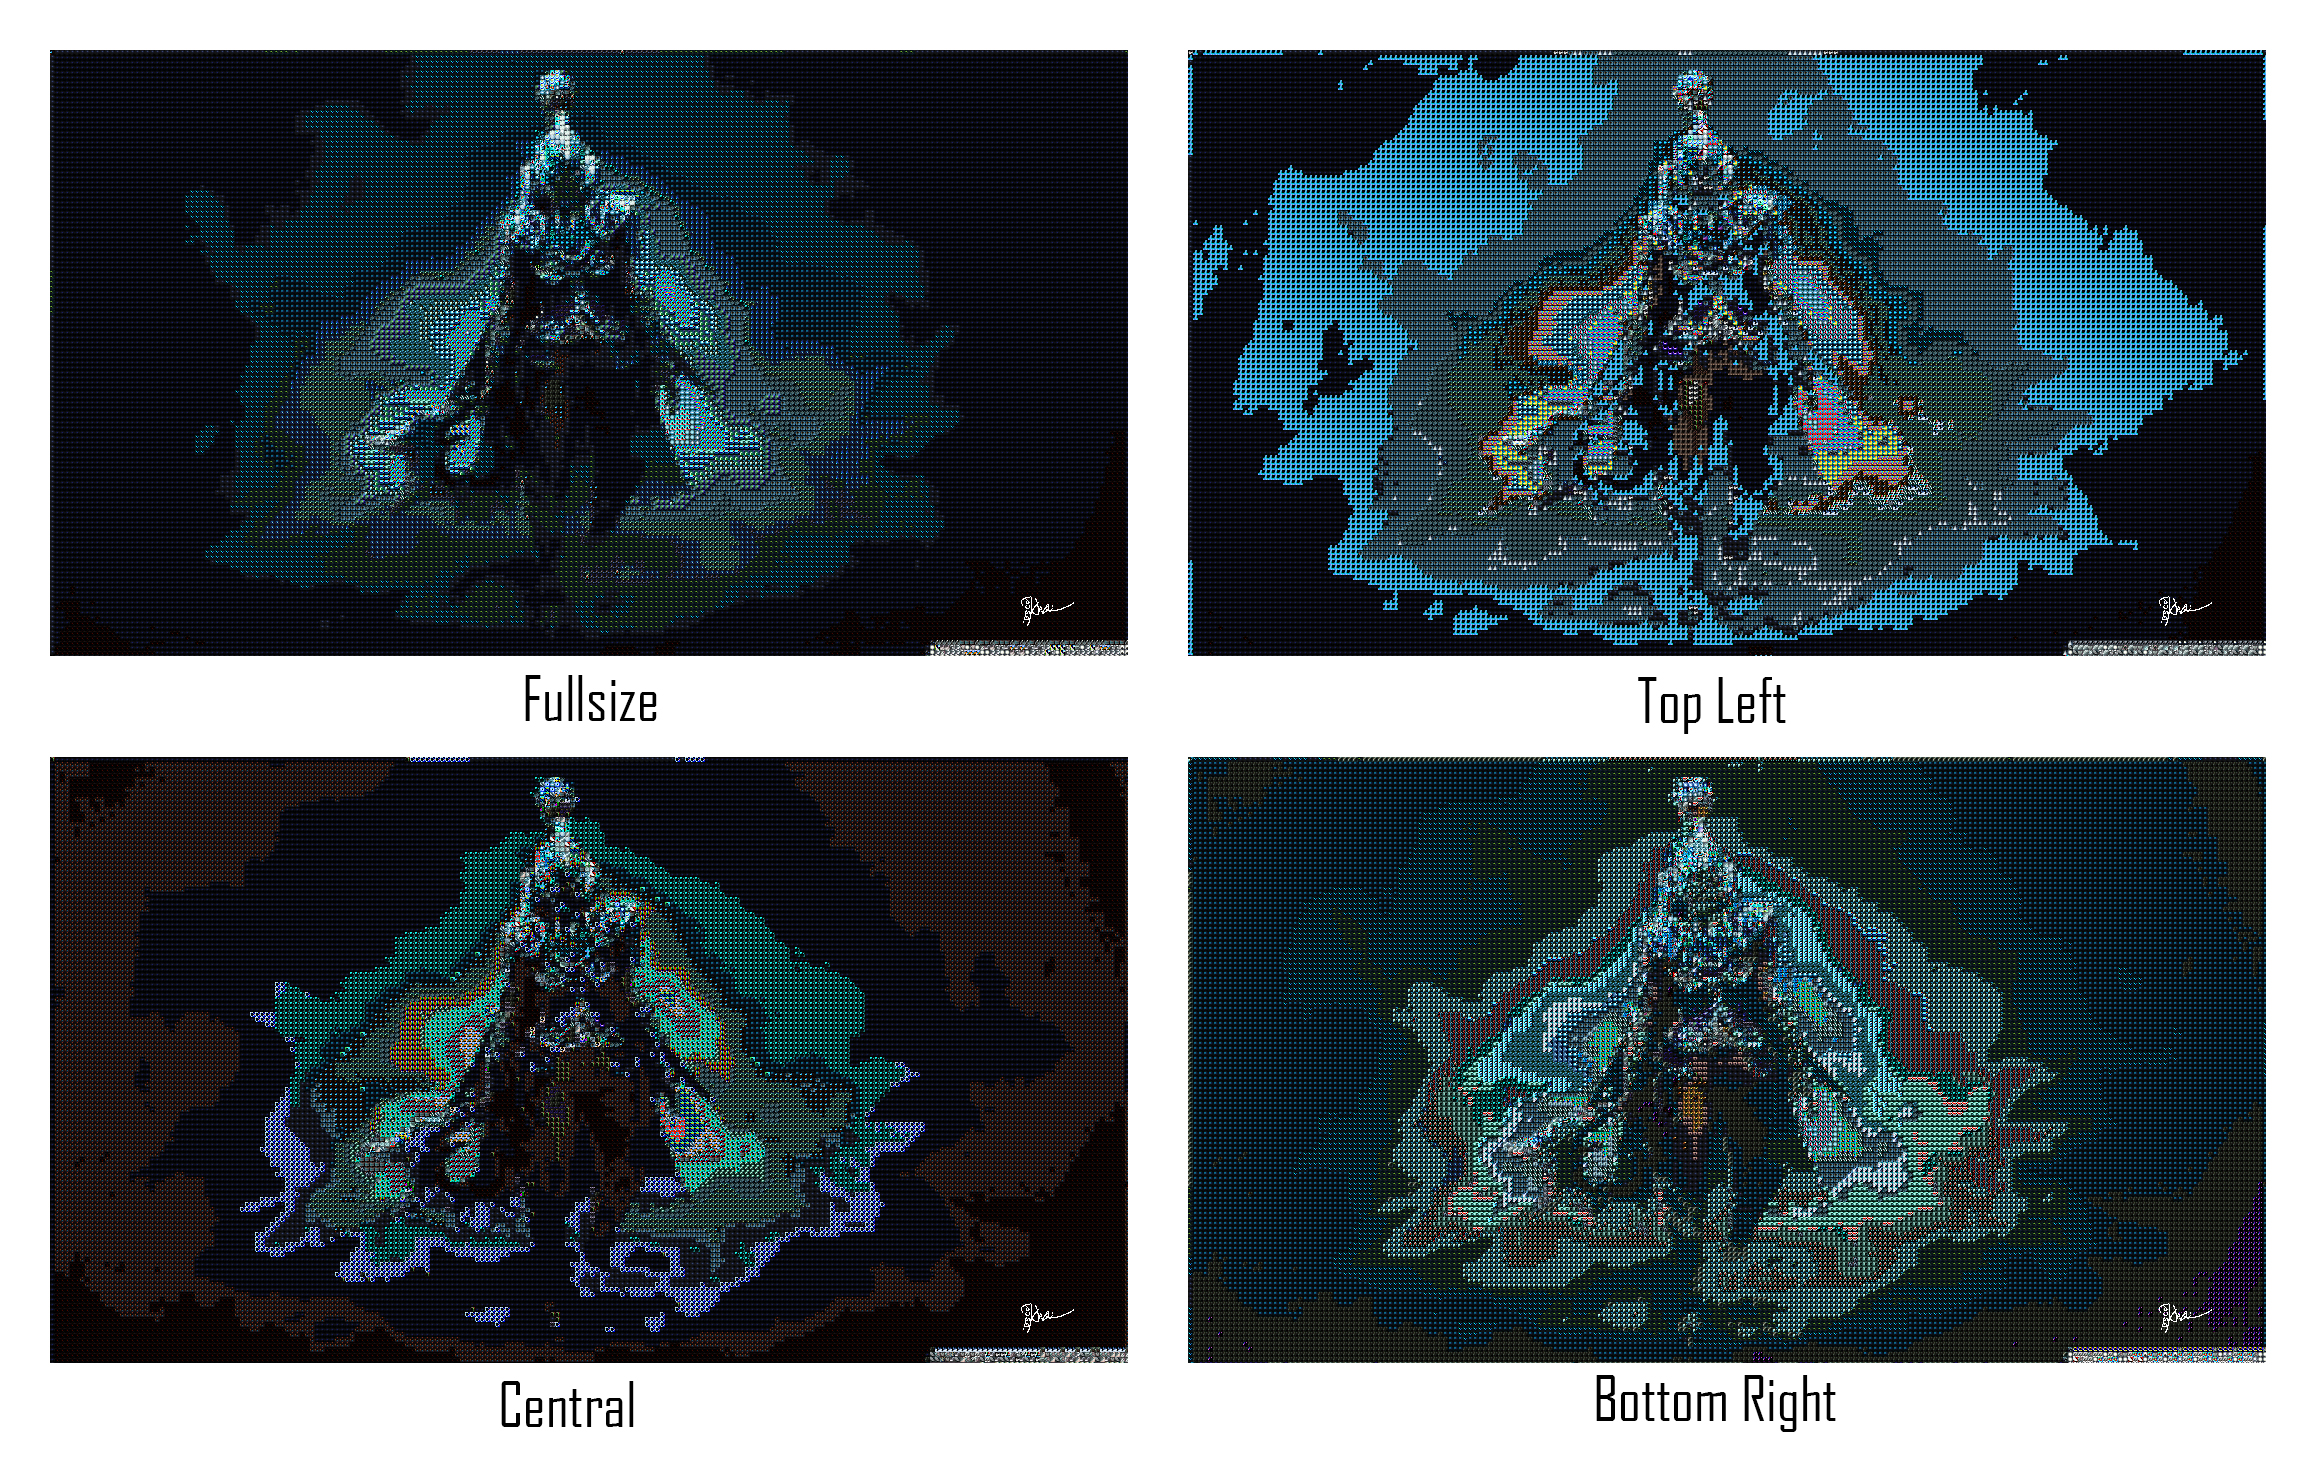
\includegraphics[width=\linewidth,height=10cm]{img/mode_demo.jpg}	
\end{center}  


Ofcourse, this feature reduces the accuracy of the findBestMatchImage() function, but to gain processing speed and the versatility of the output in trade off. We could have up to 6 different products created by 1 set of sample images.

\lstset{language=C++}
\begin{lstlisting}

	void MainWindow::on_boxMode_activated(const QString &mode){
		// 4 mark points have value from 0 to 100 (percentage). But currently they are integers,
		// I will devide them by 100 to get percentage after I pass it in the sample image process.
		// Rather than using 0, 1/4, 1/2, 3/4, I can avoid double casting this way.
		
		if(mode == "Fullsize")          { p1 = 0;   p2 = 100;   p3 = 0;     p4 =100;}
		else if(mode == "Central")      { p1 = 25;  p2 = 75;    p3 = 25;    p4 = 75;}
		else if(mode == "Top left")     { p1 = 0;   p2 = 50;    p3 = 0;     p4 = 50;}
		else if(mode == "Top right")    { p1 = 0;   p2 = 50;    p3 = 50;    p4 = 100;}
		else if(mode == "Bottom left")  { p1 = 50;  p2 = 100;   p3 = 0;     p4 = 50;}
		else if(mode == "Bottom right") { p1 = 50;  p2 = 100;   p3 = 50;    p4 = 100;}
	}
\end{lstlisting}

Above, 4 anchor point p1 p2 p3 p4 are defined according to the mode. Then I use these 4 points in the mean color extracting process of sample images as below:

\lstset{language=C++}
\begin{lstlisting}

	// set the marks point (to define the region in the sample
	// image that will be processed to compute the mean) based
	// on the width and height of the image
	int mark1 = (*sampleImage)->width()*p1/100;
	int mark2 = (*sampleImage)->width()*p2/100;
	int mark3 = (*sampleImage)->height()*p3/100;
	int mark4 = (*sampleImage)->height()*p4/100;
	
	// loop through every pixel of the sample image
	for(int m = mark1; m < mark2; ++m)
		for(int n = mark3; n < mark4; ++n){
		
			Processing..
		}
	}
\end{lstlisting}



\subsubsection{Random poses}

\begin{center}
	\includegraphics[width=3cm,height=1cm]{img/random_ui.jpg}	
\end{center} 


\begin{center}
	\includegraphics[width=5cm,height=5cm]{img/random.jpg}	
\end{center}  


This is another cool function of mine. Before the sample image get painted on the canvas, they got randomly rotated in 4 directions (0 degree, 90 degree, 180 degree and 270 degree). This way the final image get rid of same boring repeated pattern on the same color region make it looks more natural.

\lstset{language=C++}
\begin{lstlisting}
	void MainWindow::on_rdnPose_toggled(bool checked){
		checked == true ? rndPose = true : rndPose = false;
	}

\end{lstlisting}

Usage: 

\lstset{language=C++}
\begin{lstlisting}

	// rotate image randomly to prevent resemble image poses
	// will be pixelated in same color area of the original picture
	if(rndPose){
		QMatrix rm;
		int deg = (rand() % 4)*90;			  // random between 0, 1pi, 2pi, 3pi
		rm.rotate(deg);                     
		*bestImg = bestImg->transformed(rm);  // rotate img
	}

\end{lstlisting}



\subsubsection{Scaling}

This scaling algorithm is used to scale the best matched image before it get painted on the canvas. The ratio between the dimension of the sample image and dimension of the cube determined how it is scaled using scaled() function of QImage.

\lstset{language=C++}
\begin{lstlisting}

	if( bestImg->width()/cubeW <  bestImg->height()/cubeH )
	*bestImg = bestImg->scaledToWidth(cubeW);
	
	else if( bestImg->width()/cubeW >  bestImg->height()/cubeH )
	*bestImg = bestImgImg->scaledToHeight(cubeH);
	
	else
	*bestImg = bestImg->scaled(cubeW,cubeH);

\end{lstlisting}



\subsubsection{Keep sample images}

This feature save time and resource by reusing previous loaded sample images in case user want to use the same sample image folder on his next process.

\lstset{language=C++}
\begin{lstlisting}

	void MainWindow::on_sampleKeep_toggled(bool checked){
		checked == true ? keepSampleImage = true : keepSampleImage = false;
	}

\end{lstlisting}

Usage:

\lstset{language=C++}
\begin{lstlisting}

	if(!keepSampleImage){
		Open dialog choose sample image folder
		
		Processing..
		
		End sample image processing
	}
	
	Start find best matched image and pating..
\end{lstlisting}

Once the program has to deal with big size of sample images, this feature is very helpful saving tons of loading time.

\subsubsection{Watermark}

\begin{center}
	\includegraphics[width=10cm,height=3cm]{img/watermark.jpg}	
\end{center} 

A function to paint a pre-made watermark onto bottom right corner of the final picture, this function is able to detect the color range of the region where it would be painted on. Therefore, it could choose to use the appropriate version (in this case is black and white) to avoid getting into situation where the watermark fades into the picture because it has the same color with the background.

\lstset{language=C++}
\begin{lstlisting}

	// in this part I'll load the 2 versions of my watermark based on the
	// average color of the zone where I put the watermark. If the zone is
	// dark, I'll load the white watermark, otherwise I'll load the black one
	QImage *watermark = new QImage();
	
	int wtmWidth = curImg->width()/20;
	int wtmHeight = curImg->height()/20;
	
	int wtmPosX = curImg->width()-curImg->width()/10;
	int wtmPosY = curImg->height()-curImg->height()/10;
	
	// same process to calculate average color
	int wtmCount = 0, wtmR = 0, wtmG = 0, wtmB = 0, wtmA = 0, wtmTotalMean = 0;
	
	for(int x = wtmPosX; x < wtmPosX + wtmWidth; x++)
	for(int y = wtmPosY; y < wtmPosY + wtmHeight; y++){
		QColor wtmColor(artedImg.pixel(x,y));
		wtmR += wtmColor.red();
		wtmG += wtmColor.green();
		wtmB += wtmColor.blue();
		wtmA += wtmColor.alpha();
		wtmCount++;
	}
	
	wtmR /= wtmCount; wtmG /= wtmCount; wtmB /= wtmCount; wtmA /= wtmCount;
	wtmTotalMean = wtmR + wtmG + wtmB + wtmA;
	
	if(wtmTotalMean < 500)
		watermark->load("D://CProject/PixelArt/extras/wtm_w.png");   // load white watermark
	else
		watermark->load("D://CProject/PixelArt/extras/wtm_b.png");   // load black watermark
	
	// paint watermark onto the image
	cubePainter.drawImage(  QRectF(wtmPosX, wtmPosY, wtmWidth, wtmHeight),
	watermark->scaled(wtmWidth,wtmHeight),
	QRectF(0,0,wtmWidth,wtmHeight)                  );
	
	delete watermark; // free memory
\end{lstlisting}


\newpage
	
\subsection{Useful techniques / tricks}	
		
\subsubsection{QApplication::processEvents}

This technique was used to bring back the UI from freezing during long run processes. This small piece of code is placed inside loops (mainly in ArtIt function), it merely interrupt the main thread for a very short time and bring back the main thread again.\newline

Normally, this is a bad way to design a real program, every long-run process should be put in a separate thread of the processor, differ from the thread where the GUI or another function takes place. This way that long-run process could be running alone while leaving the others normally functional. \newline

However, I'm not quite familiar with C++ threading and also feel this is not so important with this kind of small program like pixelArt. Anyway, threading is always a must to design a good program.


\lstset{language=C++}
\begin{lstlisting}

	// interfere the process to unfreeze UI due to long processing time
	QApplication::processEvents();
\end{lstlisting}


\subsubsection{Free memory}

Dynamical object/instance is always the source of memory leak (the issue which the system memory still hold the object even though the program has already ended). In C++, a delete call is always required to kill that object/instance once the program doesn't need them anymore.

\lstset{language=C++}
\begin{lstlisting}
	// dynamically create an instance
	PixelCube *newcube = new PixelCube(r,g,b,a);
	
	Processing..
	
	// delete the object (prevent memory leak)
	delete newcube;
\end{lstlisting}

\lstset{language=C++}
\begin{lstlisting}
	QImage *watermark = new QImage();
	
	Processing..
	
	delete watermark;
\end{lstlisting}


\lstset{language=C++}
\begin{lstlisting}

	MinesweeperGame :: ~MinesweeperGame()
	{
		//some pixmaps might have been dynamically allocated..
		for ( int i=0; i<(int) tile_pixmaps.size(); i++ )
			delete tile_pixmaps[i];
	}
\end{lstlisting}




\end{document}
